% AER-Article.tex for AEA last revised 22 June 2011
\documentclass[AER]{AEA}

% The mathtime package uses a Times font instead of Computer Modern.
% Uncomment the line below if you wish to use the mathtime package:
%\usepackage[cmbold]{mathtime}
% Note that miktex, by default, configures the mathtime package to use commercial fonts
% which you may not have. If you would like to use mathtime but you are seeing error
% messages about missing fonts (mtex.pfb, mtsy.pfb, or rmtmi.pfb) then please see
% the technical support document at http://www.aeaweb.org/templates/technical_support.pdf
% for instructions on fixing this problem.

% Note: you may use either harvard or natbib (but not both) to provide a wider
% variety of citation commands than latex supports natively. See below.

% Uncomment the next line to use the natbib package with bibtex 
\usepackage{natbib}

%%%%%% Added packages and declarations
\RequirePackage{amsfonts,amsmath,graphicx,booktabs}

% Uncomment the next line to use the harvard package with bibtex
%\usepackage[abbr]{harvard}

% This command determines the leading (vertical space between lines) in draft mode
% with 1.5 corresponding to "double" spacing.
\draftSpacing{1.5}
\newlength\TableWidth
\usepackage{array}
\newcolumntype{H}{>{\setbox0=\hbox\bgroup}c<{\egroup}@{}}

\begin{document}

\title{In Search of Lost Time Aggregation}
\shortTitle{In Search of Lost Time Aggregation}
\author{Edmund Crawley\thanks{ Federal Reserve Board, 20th Street and Constitution Avenue N.W., Washington, DC 20551, edmund.s.crawley@frb.gov. The analysis and conclusions set forth are those of the author alone and do not indicate concurrence by other members of the research staff or the Board of Governors. Many thanks to Chris Carroll for support and guidance.}}
\date{\today}
\pubMonth{September}
\pubYear{2019}
\pubVolume{}
\pubIssue{}
\JEL{C18, D12, D31, D91, E21}
\Keywords{Income, Consumption, Time Aggregation}

\begin{abstract}
In 1960, Working noted that time aggregation of a random walk induces serial correlation in the first difference that is not present in the original series. This important contribution has been overlooked in a recent literature analyzing income and consumption in panel data. I examine \cite{blundell_consumption_2008} as an important example for which time aggregation has quantitatively large effects. Using new techniques to correct for the problem, I find the estimate for the partial insurance to transitory shocks, originally estimated to be 0.05, increases to 0.24. This larger estimate resolves the dissonance between the low partial consumption insurance estimates of \cite{blundell_consumption_2008} and the high marginal propensities to consume found in the natural experiment literature. A remaining puzzle is the low estimate I recover for the partial insurance to permanent shocks.
\end{abstract}


\maketitle

\newpage
In a short note in Econometrica, \cite{working_note_1960} made the simple but important point that time aggregation can induce serial correlation that is not present in the original series. This fact was readily absorbed by the macroeconomic literature, where time aggregated series are common\footnote{For an example see \cite{campbell_consumption_1989}} and a small literature has grown around how to account for time aggregation in various settings.\footnote{A sample of this literature includes \cite{amemiya_effect_1972}, \cite{weiss_systematic_1984} and \cite{drost_temporal_1993}.}

However, the effect of time aggregation has been overlooked in much of the  literature studying the covariance structure of household income and consumption dynamics.\footnote{The literature goes back to early work such as \cite{hause_1973}, \cite{weiss_1979} and  \cite{macurdy_time_1982} that look at the covariance structure of the income process. Following BPP, a number of papers have looked at income and consumption together, for example \cite{arellano_earnings_2017} .} This oversight can result in significant bias. I examine \cite{blundell_consumption_2008} (henceforth BPP) not only as a way to demonstrate new techniques to overcome the bias, but also because the consumption responses to transitory and permanent income shocks are of significant economic interest in themselves. Indeed, \cite{kaplan_how_2010} argue that ``the BPP insurance coefficients should become central in quantitative macroeconomics''. Using the same Panel Study of Income Dynmics (PSID) data as in BPP, I update their underlying model to account for time aggregation. I find the estimate for partial insurance to transitory shocks, originally estimated in BPP to be 0.05, to be 0.24 when time aggregation is accounted for. This new estimate resolves the dissonance between BPP's ``full insurance of transitory shocks'' and  a parallel literature that, using natural experiments, finds large consumption responses to transitory income shocks.\footnote{A small sample of this literature includes \cite{parker_consumer_2013}, \cite{agarwal_consumption_2014} and \cite{Sahmetal:2008TaxRebates}. Consumers also answer that they have a high marginal propensity to consume when asked, see \cite{fuster_what_2018} and \cite{jappelli_fiscal_2014}. For an overview of the entire literature on consumption responses to income shocks, see \cite{jappelli_consumption_2010}. Note the dissonance between BPP and the natural experiment literature is also addressed by \cite{commault_how_2017}. In contrast to this paper, her approach makes structural changes to the underlying model but does not address time aggregation.} However, a new puzzle arises from the low estimate for the partial insurance to permanent shocks, now estimated to be around 0.34. 

 While this paper will focus on the implications of time aggregation for the methodology in BPP, the techniques can be applied to a broad swath of the literature.

\begin{figure}
	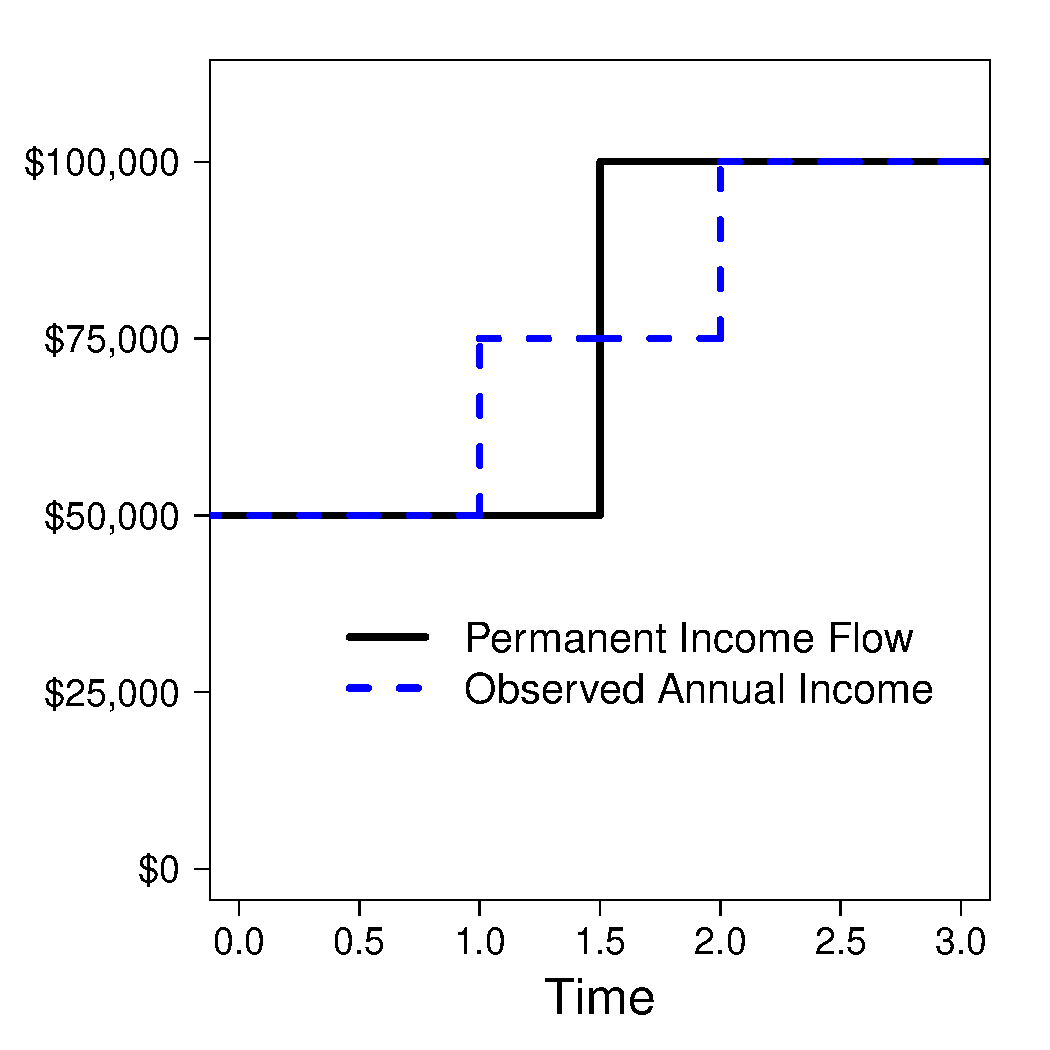
\includegraphics[width=0.7\textwidth]{../Code/Figures/TimeAgg_simple.pdf}
	\caption{Income Flow and Observed Income}
	\label{fig:TimeAggExample}
\end{figure}

\section{What is Time Aggregation?}

Time aggregation occurs when a time series is observed at a lower frequency than the underlying data that generates it. For example, income is often observed at an annual frequency when it may in fact consist of paychecks arriving at a monthly, biweekly or irregular timetable. To transform income into an annual frequency, we sum up all the income that was received by a household during the year. The key insight of \cite{working_note_1960} is that even if there is no correlation between changes in income at the underlying frequency, changes in the resulting time aggregated series will show positive autocorrelation. The intuition behind this can be seen in figure \ref{fig:TimeAggExample}, showing the income process of a household that begins with an annual salary of \$50,000 and receives a permanent pay rise to \$100,000 mid-way through the second year. The solid line shows this jump in income flow occurring just once. The crosses show the income we actually observe in annual data. During the second year the household receives an annual \$50,000 salary for six months, followed by \$100,000 in the second six months, resulting in a reported income of \$75,000 for the entire year. The single shock to income therefore appears in the time aggregated data as two increases. In this way, an income change in one year is positively correlated with an income change in the following year, even if the underlying income process follows a random walk.

\section{Modelling Time Aggregation in \cite{blundell_consumption_2008}} \label{BPP}

\subsection{The Model in Discrete Time Without Time Aggregation}
Here I briefly describe the method used  by \cite{blundell_consumption_2008} to estimate household consumption responses to permanent and transitory income shocks. The model described here is a simplified version of the original in order to highlight the role played by time aggregation.\footnote{In this simplified model I assume insurance parameters are constant across both time and households, that the transitory component of income has no persistence, and that there are no taste shocks. These elements are reintroduced in section \ref{evidence} in which I show the quantitative effect of time aggregation.} 

 The core of the model is the assumptions made on the income and consumption processes. Unexplained log income growth for household $i$ follows the process:
\begin{align*}
\Delta y_{i,t} = \zeta_{i,t} + \Delta \nu_{i,t}
\end{align*}
where $\zeta_{i,t}$ (the change in permanent income) and $\nu_{i,t}$ (transitory income) are each mean zero, finite variance, i.i.d. and independent of each other.

The unexplained change in log consumption is modeled as a random walk that moves in response to permanent and transitory income shocks:
\begin{align*}
\Delta c_{i,t} = \phi \zeta_{i,t} + \psi \nu_{i,t} 
\end{align*}
where $\phi$ and $\psi$ are the \textit{partial insurance} parameters. A value of zero implies full insurance (consumption does not respond at all to the income shock), while a value of one implies no insurance. The core of the empirical methodology is to identify these insurance parameters in the data from the following identities:
\begin{align}
\phi&= \frac{\mathrm{Cov}(\Delta c_{t}, \Delta y_{t-1}+\Delta y_{t}+\Delta y_{t+1})}{\mathrm{Cov}(\Delta y_{t}, \Delta y_{t-1}+\Delta y_{t}+\Delta y_{t+1})} \label{phi}\\
\psi&= \frac{\mathrm{Cov}(\Delta c_{t},\Delta y_{t+1})}{\mathrm{Cov}(\Delta y_{t},\Delta y_{t+1})} \label{psi}
\end{align}

\subsection{The Model in Continuous Time with Time Aggregation}
In this section I show how time aggregation can significantly bias the partial insurance parameter estimates obtained by equations \ref{phi} and \ref{psi}. The model in this section will be the exact analog of the discrete time model just described, but embedded in continuous time where shocks are spread uniformly throughout the year.\footnote{There is little formal evidence on the distribution of shocks throughout the year. While this assumption is unlikely to be strictly true, it is more reasonable than the implicit assumption of BPP that shocks all occur 1st January each year.} The main result does not hinge on the use of continuous time, and similar estimates would be obtained by dividing the year into quarters or months.\footnote{The autocorrelation of a time aggregated random walk is 0.25 in continuous time, compared to 0.23 for a discrete quarterly model and almost indistinguishable from a discrete monthly model. The theoretical moments are however significantly more elegant in continuous time. See online appendix \ref{log_tranformation}}

Time is continuous and one time unit represents one year. For the income process we will assume two underlying martingale processes, $P_t$ and $Q_t$ such that for all $s_1>s_2>s_3>s_4>0$:
\begin{align*}
\mathrm{Var}(P_{s_1}-P_{s_2})=(s_1-s_2)\sigma_P^2 \\
\mathrm{Cov}(P_{s_1}-P_{s_2},P_{s_3}-P_{s_4}) = 0 \\
P_s = 0 \qquad \text{if } s<0
\end{align*}
and similarly for $Q_t$. Brownian motion fits these assumptions, but the slightly more general definition allows for jumps in the income process. Allowing for jumps accommodates low-frequency events, such changing job or getting a promotion, that may only occur once every few years, but when they do occur they can be at any point in the year. Instantaneous income in a period $dt$ is given by:\footnote{A more formal treatment of how to relate this to the log income process is given in online appendix \ref{log_tranformation}.}
\begin{align}
dy_t = P_t dt  +dQ_t \label{income_process}
\end{align}
that is they receive their permanent income flow ($P_t =\int_{0}^{t}dP_s $) multiplied by time $dt$ in addition to a one-off transitory income $dQ_t$.

Keeping with the assumption that consumption is a random walk with insurance parameters $\phi$ and $\psi$, instantaneous consumption is given by:
\begin{align}
dc_t = \phi P_t  dt +\psi Q_t  dt  \label{consumption_process}
\end{align}
that is, they consume a proportion $\phi$ of their permanent income and a proportion $\psi$ of the cumulation of all the transitory income they have received in their lifetime  ($Q_t =\int_{0}^{t}dQ_s $).

In the Panel Study of Income Dynamics (PSID) data, we observe the total income received over the previous calendar year at time $T$:
\begin{align*}
y^{obs}_T = \int_{T-1}^{T} dy_t
\end{align*}
Consumption is measured by a survey at the beginning of the following calendar year, which I map to a snapshot of consumption exactly at the end of the calendar year:\footnote{BPP use data on food consumption to impute total annual consumption. The questionnaire asks about food consumption in a typical week, but unfortunately the timing of this `typical week' is not clear. The questionnaire is usually given at the end of March in the following year. See \cite{altonji_testing_1987} and \cite{hall_sensitivity_1982} for differing views. In online appendix \ref{interview_date} I show that controlling for the interview date barely changes the results. However, in online appendix \ref{typical_week} I show that the timing of the `typical' week can have a large effect on the results. This is an important drawback to using this method with the PSID data. In \cite{crawley_consumption_2018} we use expenditure data imputed from Danish administrative records in which the timing of expenditure is very clearly defined.}
\begin{align}
c^{obs}_T = \phi P_T  +\psi Q_T \label{c_obs}
\end{align}

The BPP method makes use of the changes in observable income and consumption, which in the time aggregated model relate to:
\begin{align}
\Delta y^{obs}_T &=  \Big(\int_{T-2}^{T-1} (s-(T-2))dP_s  + \int_{T-1}^{T} (T-s)dP_s \Big) \nonumber \\
& \qquad + \Big(\int_{T-1}^{T} dQ_t -\int_{T-2}^{T-1} dQ_t \Big) \label{deltay} \\
\Delta c^{obs}_T &= \phi  \int_{T-1}^{T} dP_s  +\psi \int_{T-1}^{T}dQ_s  \label{deltac}
\end{align}

We see that these observable income and consumption changes in equations \ref{phi} and \ref{psi} recover the permanent, but not the transitory insurance parameter:
\begin{align}
\frac{\mathrm{Cov}(\Delta c^{obs}_{T}, \Delta y^{obs}_{T-1}+\Delta y^{obs}_{T}+\Delta y^{obs}_{T+1})}{\mathrm{Cov}(\Delta y^{obs}_{T}, \Delta y^{obs}_{T-1}+\Delta y^{obs}_{T}+\Delta y^{obs}_{T+1})}&= \phi\\
%\frac{\mathrm{Cov}(\Delta c^{obs}_{T},\Delta y^{obs}_{T+1})}{\mathrm{Cov}(\Delta y^{obs}_{T},\Delta y^{obs}_{T+1})} &= \frac{-\phi\frac{1}{2}\sigma^2_P + \psi\sigma^2_Q}{-\frac{1}{6}\sigma^2_P + \sigma^2_Q} \neq \psi \label{not_psi}
\frac{\mathrm{Cov}(\Delta c^{obs}_{T},\Delta y^{obs}_{T+1})}{\mathrm{Cov}(\Delta y^{obs}_{T},\Delta y^{obs}_{T+1})} &= \psi - \frac{ (3\phi - \psi) \sigma^2_P}{6\sigma^2_Q-\sigma^2_P} \label{not_psi}
\end{align}

Indeed the transitory insurance coefficient bears little relation to the true value of $\psi$. For example, if permanent and transitory variances are equal, and households follow the permanent income hypothesis ($\phi=1$, $\psi=0$), the estimate for $\psi$ using this method will be \textit{negative} 0.6.

\section{Revised BPP Estimates} \label{evidence}

In this section I repeat the BPP estimation proceedure, but with the model moments coming from the continuous time model with time aggregated income. While the core identification in BPP is illustrated in equations \ref{phi} and \ref{psi}, the full estimation proceedure minimizes the distance between all the observable covariances ($ \mathrm{Cov}(\Delta y^{obs}_T, \Delta y^{obs}_S)$, $\mathrm{Cov}(\Delta c^{obs}_T, \Delta c^{obs}_S)$ and $\mathrm{Cov}(\Delta c^{obs}_T,  \Delta y^{obs}_S)$) and their model implied equivalents.\footnote{I follow the exact same diagonally weighted minimum distance proceedure in BPP as described in online appendix D of \cite{blundell_consumption_2008}} The full set of these model implied moments for the continuous time model, extended to include time varying coefficients, transitory persistence and taste shocks, can be found in appendix \ref{identification} and online appendix \ref{persistence_appendix}. 

\input ../Code/Tables/Persistence_short.tex

Table \ref{table:Persistence} shows the estimates for the transitory and permanent insurance parameters, first using BPP's original method and then with time aggregation. As there is no equivalent to an MA(1) process in continuous time, I consider two alternative ways to introduce persistence in the transitory shock, as well as reporting results assuming no persistence. First I assume a transitory shock provides a stream of income uniformly distributed over a short period of time (to be estimated). Second I assume the stream of income decays linearly over a short period.\footnote{See online appendix \ref{persistence_appendix} for details.} The time aggregated results are not very sensitive to these assumptions.

The top row of table \ref{table:Persistence} gives the main result showing the transitory insurance parameter increases from 0.05 in BPP to 0.24 with time aggregation. This new estimate is much more in line with the literature that estimates MPCs using natural experiments. However, the new estimate for the permanent insurance parameter is lower than before, around 0.35. This new puzzle is discussed next.

\subsection{A New Puzzle: Too Much Permanent Insurance?}
The low estimate of $\phi$ coflicts with both consumption theory and other empirical estimates.\footnote{Standard buffer stock theory suggests $\phi$ should be close to 1. The literature on consumption responses to permanent shocks is much smaller than for transitory shocks, but tends to find estimates close to 1. See  \cite{gelman_response_2016} and \cite{crawley_consumption_2018} for examples.} Furthermore, equation 8 suggests time aggregation should not alter the permanent insurance estimate, at least in the model without transitory persistence. Here I propose a further change to the model that can explain the difference observed in the permant insurance estimate between BPP and the time aggregated model. However, the low estimate for $\phi$ remains a puzzle which I suggest is a feature of the underlying Consumer Expenditure (CEX) data rather than model misspecification.

I extend the model so that, rather than consumption following a random walk, the consumption response to a transitory shock decays exponentially over time. That this consumption response decays over time is a natural consequence of a large initial response. The details are in appendix *******************. With this change, the half life of the consumption response to transitory shocks is ************, and both $\phi$ and $\psi$ are estimated to be close to 0.2. The low $\phi$ estimate is now even more of a puzzle. However, when I simulate a panel of income and consumption data from this model, using the estimated parameters, and then use this simulated panel in the original BPP algorithm, I retrieve close to the estimates in the original BPP paper. This new model specification is therefore able to explain all the differences observed in the estimations.

The low estimate of $\phi$ appears to be a feature of the data, possibly measurement error, rather than model misspecification. Indeed the relation between income and consumption in the cross-sectional CEX data is low. \cite{NBERc12673} find "The ratio of spending to income at low-income levels seems implausibly high, and the ratio of spending to income at the top seems implausibly low."  This cross-sectional relation in the CEX data is carried over to the imputed PSID consumption data used in BPP, and is reflected in the low estimates for permanent insurance.\footnote{See online appendix **************** for more detail on the low $\phi$ estimate.}

\section{Conclusion}
This paper highlights the importance of time aggregation when working with panel data, especially when analyzing the covariance matrix of income and consumption growth. It also resolves the dissonance between BPP's estimates of transitory income insurance and the natural experiment literature on marginal propensity to consume. Going forward, I hope the methods used here to correct for the time aggregation problem can be useful for researchers, especially as more and more high quality panel datasets on income and consumption become available.


% Remove or comment out the next two lines if you are not using bibtex.
\bibliographystyle{aea}
\bibliography{TimeAggEconLetters}

% The appendix command is issued once, prior to all appendices, if any.
\appendix

\section{Mathematical Appendix}
\input AppendixFullMoments.tex
\newpage
\section{For Online Publication}
\input AppendixLevelvsLogs.tex
\input AppendixTransitoryPersistence.tex
\input AppendixTypicalWeek.tex
\input AppendixExpDecay.tex

\subsection{Other Tables from the BPP paper} \label{table_appendix}

Table \ref{table:ReplicationTable} replicates Table 6 from the original BPP paper.

\input ../Code/Tables/RepTable6.tex 

Table \ref{table:ReplicationTable7} replicates Table 7 from the original BPP paper.

\input ../Code/Tables/RepTable7.tex 

Table \ref{table:ReplicationTable8} replicates Table 8 from the original BPP paper.\input ../Code/Tables/RepTable8.tex


\end{document}

